\documentclass[10pt, openany]{article}

\usepackage{needspace} % assicura che ci sia spazio di almeno tot per la prossima section
\usepackage{placeins} % per la \FloatBarrier
\usepackage{adjustbox} % per l'adjust box, che fa il frame e trasforma grafici
\usepackage{graphicx}
\usepackage{xcolor} % per definire i colori con definecolor
\usepackage{mdframed} % provo a fare boxing di figures con mdframed
\usepackage{longtable} % tabella degli assets va oltre una pagina
\usepackage{caption}
\usepackage{subcaption}
\usepackage{enumitem}
\usepackage{listings}
\lstdefinestyle{sharpc}{
  language=[Sharp]C, 
  basicstyle=\ttfamily\small,
}

\definecolor{gray80}{rgb}{0.2,0.2,0.2} % 80% black
\definecolor{gray60}{rgb}{0.4,0.4,0.4} % 60% black

\lstdefinelanguage{TOML}{
  comment = [l]{\#},
  keywords = {true, false, [, ]},
  morestring = [b]{"}
}

\lstdefinestyle{toml}{
  language=TOML, % No specific language
  basicstyle=\ttfamily\small, % Default text style
  tabsize = 2,
  frame = single,
  breaklines = true,
  %numbers = left,
  %numbersep = 5pt,
  %numberstyle = \color{white!30!black}\scriptsize,
  %stepnumber = 1,
  escapeinside={/*}{*/}, % For inline LaTeX commands if needed
  basicstyle = \footnotesize\ttfamily,
  commentstyle={\color{gray60}\ttfamily},
  keywordstyle = {\bfseries\color{purple}}, % keywords
  keywordstyle = [2]{\itshape\color{blue}}, % traits
  keywordstyle = [3]{\color{blue}}, % primitive types
  keywordstyle = [4]{\color{blue}}, % type and value ctors
  keywordstyle = [5]{\color{purple!50!blue}}, % macros
  stringstyle = \color{gray80!80!green},
  aboveskip = \baselineskip,
  showstringspaces = false
}

\usepackage{tikz}
\usepackage[colorlinks=true, linkcolor=blue, urlcolor=blue]{hyperref}
\usepackage{geometry}
\geometry{
  a4paper,
  total={170mm,257mm},
  left=20mm,
  top=20mm,
}

\usepackage{booktabs} % per midrule, toprule, bottomrule
\usepackage{multirow} % multiriga multicolonna in tabelle
\usepackage{array} % per colonne paragrafo con size fissa
\usepackage{pdflscape} % per le pagine orizzontali, landscape

% roba per grafiche
\usepackage{pgf}
\usepackage{tikz}
\usetikzlibrary{arrows, arrows.meta} % arrow stile stealth
\usetikzlibrary{positioning} % positioning con of
\usetikzlibrary{fit, shapes.geometric} % per racchiudere il blocco game paused
\usetikzlibrary{umlcd} % UML Diagrams
\tikzset{
  state/.style={
    rectangle,
    rounded corners,
    draw=black, very thick,
    minimum height=2em,
    inner sep=2pt,
    text centered,
  },
}

\lstnewenvironment{egdlisting}
{\minipage{\dimexpr 0.48\textwidth}}
{\endminipage}

% Possibili titoli:
% "The War Arsenal: Italy's WWI Journey"
% "Echoes of Conflict: Italy's WWI Museum"
% "Frontline Relics: Italy in WWI"
% "The Weaponry of History: Italy in WWI"
% "War and Memory: Italy’s WWI Museum"
% "Artifacts of War: Italy’s WWI Story"
% "Battlefront Relics: The Italian WWI Museum"
% "Steel and Stone: Italy's WWI Legacy
% nome in codice: WW1 VR Museum

\renewcommand*\contentsname{Indice}
\begin{document}
  \begin{titlepage}
    \begin{center}
      {\Huge\textbf{WW1 VR Museum}} \\[1cm]
      {\Large\textit{Progetto Realt\`a Virtuale}} \\[2cm]
      \vfill
    \end{center}
    \hfill
    % Manca un logo o una immagine qualsiasi qui
    \begin{minipage}[t]{0.4\textwidth}
      \raggedleft
      \textbf{Team Members:} \\
      Tanzi	Alessio \\
      De Luca Giorgia \\
      Di Gregorio	Antonino \\
      Esteves Duart Vincent \\
    \end{minipage}
    \vfill
    \begin{center}
      {\large Documento di Design}
    \end{center}
  \end{titlepage}
  \tableofcontents
  \section{Obiettivi}
    L'applicazione virtuale codename \textit{WW1 VR Museum} si pone l'obiettivo di educare e sensibilizzare, in modo
    pi\`u coinvolgente e interattivo, l'utente alle vicende della prima guerra mondiale dal punto di vista dello stato italiano, 
    concentrandosi sulle vicende avvenute nei dintorni del Comune di Gorizia, cittadina il cui museo, "Museo della Grande Guerra", \`e 
    il riferimento principale per l'ambiente riprodotto.\par
    Il suddetto coinvolgimento verr\`a realizzato attraverso l'inclusione, per ogni artefatto in mostra, di modalit\`a di interazione
    multisensoriali quali contenuti audio-visivi e manipolazione dei reperti rappresentanti la tecnologia bellica dell'alba del XX secolo.
  \section{Applicazioni preesistenti nel settore}
    da fare
  \section{User Experience}\label{vr:ux}
    \subsection{Sistema di Movimento}
    L'applicazione \`e progettata come una esperienza in \textbf{prima persona}, rivestendo i panni di un visitatore del museo riprodotto.
    Ci\`o sottointende che il sistema di movimento si limita a rappresentare la \textbf{camminata} dell'utente nelle varie sale di esposizione.\par
    \subsection{Interazioni}\footnote{Rappresentate in forma grafica in seguito}
    Ciascuna sala del museo contiene uno o pi\`u oggetti di interesse storico, i quali chiamiamo d'ora in poi \texttt{Interaclables}, mentre chiamiamo 
    il centro di massa rappresentante l'utente \textit{Player Pawn}. Ogni 
    Interactable pu\`o essere ispezionato dall'utente se le seguenti condizioni sono soddisfatte:
    \begin{itemize}[noitemsep, topsep=0pt]
      \item \textbf{Vicinanza}: l'\textit{Interaclable} si trova a meno di una distanza di threshold prefissata dal \textit{Player Pawn}.
      \item \textbf{Line of Sight non ostruita}: la linea d'aria che collega il \textit{Player Pawn} al Bounding Box dell'interactable non trova nel suo 
        cammino altre ostruzioni.
      \item \textbf{Puntamento}: La direzione forward della camera associata all'utente si trova al di sotto di un displacement massimo 
        dal centro di massa del bounding box dell'\textit{Interactable}. Tale displacement \`e misurato nel piano passante per il centro di massa 
        del suddetto perpendicolare alla direzione forward della camera.\par
        In caso pi\`u \textit{Interaclables} soddisfano le prime due condizioni, quello scelto per una potenziale interazione, e comunicato attraverso un 
        feedback visivo quale \textit{Outline}, \`e quello avente displacement minimo.
      \item \textbf{Interazione}: Se le tre condizioni soprascritte sono soddisfatte, allora alla pressione della Input Action
        \textit{Interact}\footnote{Tutte le actions sono dettagliate in sottoparagrafo \ref{vr:commands}}, l'evento, da noi chiamato d'ora in poi \textit{Interaction}, viene lanciato.
    \end{itemize}
    \begin{landscape}
    \begin{table}[h!]
      \centering
      \begin{tabular}{@{} p{0.15\paperheight} p{0.3\paperheight} p{0.25\paperheight} @{}}
        \toprule
        \textbf{\textit{Interactable} Type} & \textbf{Effetto su \textit{Interaction}} & \textbf{VR vs Desktop} \\
        \midrule
        \textit{UI Interactable} & 
        Visualizzazione di uno \textit{Screen-Aligned Billboard}\footnotemark[3] contenente del testo formattato 
        atto a fornire una descrizione dell'\textit{Interactable}, d'ora in poi li chiamiamo \textit{UI Billboard}. A ciascun paragrafo mostrato 
        viene associata una audio riproducibile attraverso un Play Button facente parte della UI del Billboard mostrato. L'\textbf{allontanamento}, oltre un certo 
        threshold, dell'utente dall'\textit{Interactable}, o il lancio di un altro evento \textit{Interaction}, causano la chiusura della sessione di 
        interazione con l'\textit{UI Interactable corrente}.
        & \begin{itemize}[topsep=0pt, noitemsep]
          \item[\textbf{VR}]: Billboard compare in una posizione e orientamento variabile, specificata come un offset da posizione e orientamento corrente dell'HMD.
          \item[\textbf{DT}]: Billboard compare in una posizione e orientamento fissa, specificata come un offset da posizione e orientamento dell'\textit{Interactable}.
        \end{itemize} \\
        
        \textit{Tinkerable Interactable} & 
        L'oggetto viene spostato davanti all'utente\footnotemark[4] e viene fissato in una posizione "a mezz'aria".\par
        Viene mostrato uno \textit{UI Billboard} relativo alle generalit\`a dell'oggetto.\par
        Il \textit{Tinkerable Interactable} \`e costituito da pi\`u \textit{Interactables} i quali possono essere manipolati spazialmente tramite la successione delle 
        Input Actions \textit{Dismantle}, \textit{Interact} e \textit{Rotate}\footnotemark[5].\par
        Le condizioni di chiusura della sessione di interazione sono diverse rispetto a quelle di un \textit{UI Interactable}, dettagliate nella colonna successiva.
        & \begin{itemize}[topsep=0pt, noitemsep]
          \item[\textbf{VR}]: L'utente conclude la sessione di interazione muovendosi con la Primary 2D Axis del Left Hand XR Controller (Vedi sottoparagrafo \ref{vr:commands}).\par
          Il moto fisico dell'utente non viene contato.\par
          Ciascun \textit{Interactable} costituente \`e solidale con la mano che funge da ancora.
          \item[\textbf{DT}]: L'utente conclude la sessione di interazione alla pressione di una delle keys riservate al movimento (Vedi sottoparagrafo \ref{vr:commands}).\par
          Ciascun \textit{Interactable} costituente \`e fisso.
        \end{itemize} \\
        
        \textit{Sequence Interactable} & 
        Avvia una animazione predefinita, costituita dal keyframing delle varie mesh che compongono l'\textit{Interactable} in esame.\par
        Inoltre, comporta l'apparizione di una \textit{UI Billboard}\footnotemark[6], 
        la quale, oltre a possedere la solita spiegazione audiovisiva, fornisce anche elementi UI per il restart dell'animazione.\par
        Le condizioni di chiusura della sessione di interazione sono le stesse di un \textit{UI Interactable}.
        & \\

        \bottomrule
      \end{tabular}
      \caption{Ogni qual volta emerga evento \textit{Interaction}, l'oggetto \textit{Interactable} interessato risponde a tale evento in maniera dipendente dal tipo
        di interazione configurata per tale oggetto.
        Sono stati individuati tre possibili tipologie di interazione, dettagliate graficamente in seguito, qui elencate}
    \end{table}
    \end{landscape}
    \footnotetext[3]{citazione necessaria}\footnotetext[4]{eventuale riorientamento della camera se non vi \`e presente spazio necessario davanti all'utente per ospitare l'oggetto}
    \footnotetext[5]{Dettagliato in seguito}\footnotetext[6]{Dunque \textit{Sequence Interactable} \`e una sottoclasse di \textit{UI Interactable}}
    \setcounter{footnote}{6}
    \subsection{VR vs Desktop: Input Actions Mapping}\label{vr:commands}
    Ciascuna delle seguenti \textit{Input Actions} corrispondono ad un determinato Mapping nello schema dei comandi, e causa un effetto diverso nella simulazione a 
    seconda dello stato attuale dell'utente (dettagliato in seguito)
    \begin{table}[h!]
      \centering
      \begin{tabular}{@{} p{0.2\textwidth} p{0.4\textwidth} p{0.4\textwidth} @{}}
        \toprule
        \textbf{Input Actions} & \textbf{OpenXR Mapping} & \textbf{Desktop Mapping} \\
        \midrule
        \textit{Move} & (Left Hand XR Controller) Primary 2D Axis, (XR HMD) Center Eye Position & (Keyboard) WASD Keys \\
        \textit{Tilt} & (XR HMD) Center Eye Rotation & (Mouse) Mouse X, Mouse Y Axes \\
        \textit{Interact} & (Left Hand XR Controller) Grip Button, (Right Hand XR Controller) Grip Button & (Keyboard) F o (Mouse) LMB \\
        \textit{Dismantle} & (Left Hand XR Controller) Trigger, (Right Hand XR Controller) Trigger & (Keyboard) T o (Mouse) RMB \\
        \textit{Assemble} & (Left Hand XR Controller) Trigger, (Right Hand XR Controller) Trigger & (Keyboard) T o (Mouse) RMB \\
        \textit{Grab} & [(Left Hand XR Controller) Grip Button o (Right Hand XR Controller) Grip Button] & (Mouse) LMB \\
        \textit{Throw} & [(Left Hand XR Controller) Grip Button o (Right Hand XR Controller) Grip Button] & (Mouse) LMB \\
        \textit{Rotate} & [(Left Hand XR Controller) Grip Button o (Right Hand XR Controller) Grip Button]\footnotemark 
          + movimento "Circle-Like" Left Hand XR Controller & (Mouse) LMB + (Mouse) Mouse X, Mouse Y Axes \\
        % serve lo stato giusto. Dopo un po' di inattivita in quello stato l'oggetto ruota da solo attorno alla global y
        \textit{ResetRotation} & (Left Hand XR Controller) Trigger, (Right Hand XR Controller) Trigger & (Keyboard) T o (Mouse) RMB \\ 
        \textit{Pause} & (Left Hand XR Controller) Primary Button, (Right Hand XR Controller) Primary Button & (Keyboard) ESC \\
        \textit{CloseMenu} & (Left Hand XR Controller) Primary Button, (Right Hand XR Controller) Primary Button & (Keyboard) ESC \\
        \bottomrule
      \end{tabular}
      \caption{Soggetta al cambiamento man mano che lo sviluppo prosegue}
    \end{table}
    \footnotetext{mentre una mano afferra l'oggetto, l'altra pu\`o ruotarlo}
    \subsection{Interazione: Actions, States, Effects}
    La dinamica di interazione \`e modellabile attraverso la specifica della terna
    \begin{itemize}[leftmargin=15mm, topsep=0pt, noitemsep]
      \item[\textbf{Actions}] I trigger per una transizione di stato. Possono essere essenzialmente di due tipi
        \begin{itemize}[topsep=0pt, noitemsep]
          \item \textit{Input Actions} compiute dall'utente attraverso i vari Mapping ad uno schema di comandi, dettagliato nel sottoparagrafo precedente.
          \item \textit{Game Actions} attivate sotto condizioni specifiche legate alla logica di gioco e non direttamente all'input dell'utente
        \end{itemize}
      \item[\textbf{States}] I possibili stati in cui l'utente si pu\`o trovare all'interno della simulazione.
      \item[\textbf{Effects}] Procedure eseguite durante una transizione di stato causata da una Action.
    \end{itemize}
    Di seguito la lista delle \textit{Game Actions}
    \begin{table}[h]
      \centering
      \begin{tabular}{@{} p{0.2\textwidth} p{0.8\textwidth} @{}}
        \toprule
        \textbf{Game Actions} & \textbf{Descrizione} \\
        \midrule
        \textit{CrossCloseDistance} & Nello stato \textit{UIView}, l'utente si allontana oltre un predeterminato threshold dall'\textit{UI Interactable} con il quale \`e
          ingaggiato in una sessione di interazione. \\
        \textit{MovementBreak} & In uno stato \textit{Tinker}, l'utente cerca di muoversi, chiudendo la sessione di interazione. In desktop, \`e sufficiente 
          pigiare un tasto per il moto. In HMD VR, bisogna attivare la \textit{Input Action} con \textit{Left Hand XR Controller} Primary 2D Axis, e non con 
          la (XR HMD) Center Eye Position \\
        \textit{ClickMenu} & Nello stato \textit{GamePaused}, tale action viene lanciata ogni qual volta si interagisce con un \textit{UI Button} del menu di pausa. In modalit\`a
          desktop, tale bottone \`e determinato dai vari bouding boxes dei bottoni e le coordinate del click, mentre in modalit\`a HMD VR, dove gli \textit{UI Button}s sono
          disposti nelle direzioni cardinali solidali al Right Hand XR Controller, il valore delle (Right Hand XR Controller) Primary 2D Axis al momento del click del pulsante
          (Right Hand XR Controller) Primary 2D Axis Button determina il bottone premuto. \\
        \bottomrule
      \end{tabular}
    \end{table}
    Di seguito la lista di possibili stati in cui l'utente si pu\`o trovare
    \begin{table}[h]
      \centering
      \begin{tabular}{@{} p{0.2\textwidth} p{0.8\textwidth} @{}}
        \toprule
        \textbf{State} & \textbf{Descrizione} \\
        \midrule
        \textit{Roaming} & L'utente non \`e ingaggiato in nessuna sessione di interazione, ed \`e dunque in perlustrazione libera degli ambienti virtuali del 
          museo \\
        % puoi focusare un UI billboard anche da tinkerDismantled
        \textit{UIView} & L'utente sta correntemente visualizzando lo \textit{UI Billboard} associato ad uno \textit{UI Interactable} o un \textit{Sequence Interactable} \\
        \textit{TinkerView} & L'utente sta correntemente visualizzando uno \textit{Tinkerable Interactable} assieme al suo \textit{UI Billboard} d'insieme associato \\
        \textit{TinkerDismantled} & L'utente sta correntemente visualizzando uno \textit{Tinkerable Interactable} "Esploso" nei suoi \textit{Interactable}s costituenti, 
          distribuiti spazialmente in maniera pseudocasuale tenendo in considerazione l'ambiente circostante libero disponibile \\
        \textit{TinkerComponent} & L'utente ha afferrato un \textit{Tinkerable Interactable} (da \textit{TinkerView}) o un suo \textit{Interactable} costituente 
          (da \textit{TinkerDismantled}), ed \`e capace, oltre a visualizzare ed interagire con la sua \textit{UI Billboard} associata, a ruotare l'oggetto \\
        \textit{GamePaused} & viene visualizzata la UI corrispondente al menu di pausa, e pu\`o dunque interagire con ciascuno dei pulsanti attraverso "Punta e Clicca"
          in modalit\`a desktop (menu mostrato come layer a sovraimpressione della viewport di gioco), oppure attraverso Primary 2D Axis Touch + Primary Axis 2D (bottoni mostrati 
          solidali alla mano che ha premuto il tasto di pausa, nelle quattro direzioni cardinali. Dunque il tocco in una posizione spaziale del 
          touchpad\footnotemark permette il riconoscimento del bottone di UI premuto). \\
        \bottomrule
      \end{tabular}
    \end{table}
    \footnotetext{Caso HTC Vive Wand Controller}
    Di seguito la lista di possibili effetti lanciati a seguito di una Input Action.\par 
    Dalle specifiche soprascritte, possiamo derivare un diagramma a stati che sintetizza le interazioni utente con gli \textit{Interactables} 
    del museo (vedi Tabella \ref{vr:states}).
    \begin{landscape}
    \begin{table}[h]\label{vr:states}
      \centering
      \begin{tabular}{@{} p{0.13\paperheight} p{0.73\paperheight} @{}}
      \toprule
      \textbf{Effect} & \textbf{Matrice Stato Azione} \\
      \midrule
      \textit{ChangePosition} & \begin{tabular}{@{} l|p{0.6\paperheight}@{}}
        \textbf{Stato/Azione} & \textit{Move} \\
        \midrule
        \textit{Roaming} & traslazione \textit{Player Pawn} \\
        \textit{UIView} & traslazione \textit{Player Pawn} \\
        \textit{GamePaused} & solo in modalit\`a HMD VR, traslazione \textit{Player Pawn} \\
        \midrule
        \end{tabular} \\
      \textit{ChangeOrientation} & \begin{tabular}{@{} l|p{0.6\paperheight}@{}} 
        \textbf{Stato/Azione} & \textit{Tilt} \\
        \midrule
        (tutti tranne a seguire) & rotazione orientamento \textit{Player Pawn} \\
        \textit{TinkerView} & effetto soprascritto solo in modalit\`a HMD VR \\
        \textit{TinkerDismantled} & effetto soprascritto solo in modalit\`a HMD VR \\
        \textit{TinkerComponent} & effetto soprascritto solo in modalit\`a HMD VR \\
        \textit{GamePaused} & effetto soprascritto solo in modalit\`a HMD VR \\
        \midrule
        \end{tabular} \\
      \textit{ShowUI} & \begin{tabular}{@{} l|p{0.3\paperheight} p{0.3\paperheight} @{}} 
        \textbf{Stato/Azione} & \textit{Interact(UIInteractable)} & \textit{Interact(TinkerableInteractable)} \\
        \midrule
        \textit{Roaming} & istanziazione di un \textit{UIBillboard} con transform e contenuto iniziale determinati rispettivamente dalla modalit\`a (HMD VR o Desktop, vedi paragrafo 
          comandi) e dalla descrizione di markup associata allo \textit{UIInteractable}. Lo \textit{UIBillboard} possiede un tasto di chiusura.
                         & istanziazione di un \textit{UIBillboard} con transfomr e contenuto iniziale determinati rispettivamente da un offset dal \textit{TinkerableInteractable} e 
          dalla descrizione di markup associata allo stesso. Inoltre, sono istanziati dei bottoni per ogni \textit{UIInteractable} che lo costituisce.\footnotemark[9]. 
          Lo \textit{UIBillboard} \textit{non} possiede un tasto di chiusura. \\
        \midrule
        \end{tabular} \\
      \textit{CloseUI} & \begin{tabular}{@{} l|p{0.2\paperheight} p{0.2\paperheight} @{}} 
        \textbf{Stato/Azione} & \textit{MovementBreak} & \textit{Interact(UIBillBoard)}\footnotemark[10] \\
        \midrule
        \textit{UIView} & & Alla pressione dei tasto di chiusura, viene distrutto il \textit{UIBillBoard} associato all'\textit{UIInteractable}, e viene chiusa la sessione di 
          interazione, passando allo stato \textit{Roaming} \\
        \textit{TinkerView} & Riposizionamento del \textit{TinkerableInteractable} e distruzione del \textit{UIBillBoard} e di tutti gli \textit{UIRadio} & \\
        \textit{TinkerDismantled} & Dopo effetto \textit{ResetPieces}, del \textit{TinkerableInteractable} e poi prosegui come specificato in riga sopra. & \\
        \textit{TinkerComponent} & Come riga sopra. & \\
        \midrule
        \end{tabular} \\
      \bottomrule
      \end{tabular}
    \end{table}
    \end{landscape}
    \begin{landscape}
    \begin{table}[h]
      \centering
      \begin{tabular}{@{} p{0.13\paperheight} p{0.73\paperheight} @{}}
      \toprule
      \textbf{Effect} & \textbf{Matrice Stato Azione} \\
      \midrule
      \textit{ShowMenu} & \begin{tabular}{@{} l|p{0.6\paperheight} @{}} 
        \textbf{Stato/Azione} & \textit{Pause} \\
        \midrule
        (tutti) & Istanziazione o Cambio visibilit\`a degli \textit{UIButton} costituenti il menu di pausa "principale", e quindi transiziona allo stato \textit{GamePaused}. \`E 
          necessario memorizzare lo stato di partenza. \\
        \midrule
        \end{tabular} \\
      \textit{HideMenu} & \begin{tabular}{@{} l|p{0.6\paperheight} @{}} 
        \textbf{Stato/Azione} & \textit{CloseMenu} \\
        \midrule
        \textit{GamePaused} & Distruzione o Cambio visibilit\`a degli \textit{UIButton} costituenti il menu di pausa, e torna al menu di pausa "principale" nell'ultimo caso. Infine, 
          transiziona allo stato antecedente alla pausa. \\
        \midrule
        \end{tabular}\\
      \textit{MenuEffect} & \begin{tabular}{@{} l|p{0.6\paperheight} @{}} 
        \textbf{Stato/Azione} & \textit{ClickMenuUI(UIButton)} \\
        \midrule
        \textit{GamePaused} & Esegue una logica associata allo \textit{UIButton}, ad esempio chiusura del gioco, mostra altri pulsanti del menu di pausa, ... \\
        \midrule
        \end{tabular} \\
      \textit{OpenTinkerView} & \begin{tabular}{@{} l|p{0.6\paperheight} @{}} 
        \textbf{Stato/Azione} & \textit{Interact(TinkerableInteractable)} \\
        \midrule
        \textit{Roaming}\footnotemark[11] & Posizionamento del \textit{TinkerableInteractable} nella posizione di destinazione, ad un dato offset dalla
          posizione del \textit{PlayerPawn} \\
        \midrule
        \end{tabular} \\
      \textit{CloseTinkerView} & \begin{tabular}{@{} l|p{0.6\paperheight} @{}} 
        \textbf{Stato/Azione} & \textit{MovementBreak} \\
        \midrule
        \textit{TinkerView} & In seguito all'effetto \textit{CloseUI}, riposiziona il \textit{TinkerableInteractable} nella sua posizione iniziale e transiziona nello stato 
          \textit{Roaming} \\
        \textit{TinkerDismantled} & In seguito agli effetti \textit{ResetPieces}, \textit{CloseUI}, esegui lo stesso compito a riga sopra. \\
        \textit{TinkerComponent} & Analogo a riga sopra. \\
        \midrule
        \end{tabular} \\
      \textit{ScatterPieces} & \begin{tabular}{@{} l|p{0.6\paperheight} @{}} 
        \textbf{Stato/Azione} & \textit{Dismantle} \\
        \midrule
        \textit{TinkerView} & Distribuisce, nello spazio disponibile alla posizione corrente del \textit{TinkerableInteractable}, ciascun suo componente (\textit{UIInteractable}), e
          quindi transiziona nello stato \textit{TinkerDismantled} \\
        \midrule
        \end{tabular} \\
      \textit{ResetPieces} & \begin{tabular}{@{} l|p{0.6\paperheight} @{}} 
        \textbf{Stato/Azione} & \textit{Assemble} \\
        \midrule
        \textit{TinkerDismantled} & Riposiziona tutti i componenti (\textit{UIInteractable}) che costituiscono il \textit{TinkerableInteractable}, nelle loro posizioni originali, e dunque
          transiziona allo stato \textit{TinkerView} \\
        \midrule
        \end{tabular} \\
      \textit{FocusComponent} & \begin{tabular}{@{} l|p{0.6\paperheight} @{}} 
        \textbf{Stato/Azione} & \textit{Grab(UIInteractable)} \\
        \midrule
        \textit{TinkerDismantled} & Posiziona l'elemnento selezionato nella posizione di ancoraggio. Nel caso HMD VR, corrisponde alla mano che ha eseguito l'azione, mentre in Desktop si
          tratta di una posizione predefinita. \\
        \midrule
        \end{tabular} \\
      \textit{DeFocusThrow} & \begin{tabular}{@{} l|p{0.6\paperheight} @{}} 
        \textbf{Stato/Azione} & \textit{Throw(UIInteractable)} \\
        \midrule
        \textit{TinkerComponent} & Riposiziona il componente in aria applicandogli una forza impulsiva, e abilitando momentaneamente la gravit\`a, la cui intensit\`a \`e fissa in 
          caso Desktop, e proporzionale all'accelerazione istantanea al momento del lancio nel caso HMD VR. Quindi transiziona allo stato \textit{TinkerDismantled} \\
        \midrule
        \end{tabular} \\
      \textit{TransformInteractable} & \begin{tabular}{@{} l|p{0.3\paperheight} p{0.3\paperheight} @{}} 
        \textbf{Stato/Azione} & \textit{Rotate(UIInteractable)} \\
        \midrule
        \textit{TinkerComponent} & Applica una rotazione allo \textit{UIInteractable} ancorato, la cui asse di rotazione \`e determinata dallo spostamento del mouse, o Controller, 
          dalla pressione del tasto associato alla azione. 
                                 & Reset dell'orientamento iniziale del \textit{UIInteractable} \\
        \midrule
        \end{tabular} \\
      \bottomrule
      \end{tabular}
    \end{table}
    \end{landscape}
    \begin{landscape}
    \begin{table}[h]
      \centering
      \begin{tabular}{@{} p{0.13\paperheight} p{0.73\paperheight} @{}}
      \toprule
      \textbf{Effect} & \textbf{Matrice Stato Azione} \\
      \midrule
      \textit{TransformUI} & \begin{tabular}{@{} l|p{0.15\paperheight} p{0.15\paperheight} p{0.15\paperheight} p{0.15\paperheight} @{}} 
        \textbf{Stato/Azione} & \textit{Interact(UIBillboard)} & \textit{Interact(UIRadio)} & \textit{Grab(UIInteractable)} & \textit{Throw(UIInteractable)}\\
        \midrule
        \textit{UIView} & In seguito al click di un pulsante nell'ologramma testuale, viene eseguita l'azione corrispondente all'elemento ui cliccato, ad esempio espandi/comprimi 
          paragrafo, play/pause audio associato al paragrafo & \\
        \textit{TinkerView} & Interagisci con lo \textit{UIBillboard} associato al \textit{TinkerableInteractable} in modo analogo all'interazione con \textit{UIInteractable} nello 
          stato \textit{UIView} 
                            & Trasforma la posizione e cambia il contenuto dello \textit{UIBillBoard} a seconda dello \textit{UIInteractable} associato al \textit{UIRadio} premuto. \\
        \textit{TinkerDismantled} & & Analogo alla riga qui sopra. 
                            & Dopo effetto \textit{FocusComponent}, riposiziona il \textit{UIBillboard} associato al \textit{TinkerableInteractable} e mostra il contenuto 
                              associato al componente selezionato & \\
        \textit{TinkerComponent} & Analogo a due righe qui sopra, applicato al testo associato al componente \textit{UIInteractable} in esame & & 
                            & Dopo effetto \textit{DeFocusThrow}, ripristina tutti i \textit{UIRadio} nascosti e sposta il \textit{UIBillBoard} nella sua posizione iniziale, 
                              reinserendo il testo associato al \textit{TinkerableInteractable} \\
        \midrule
        \end{tabular} \\
      \textit{TransformUI} & \begin{tabular}{@{} l|p{0.6\paperheight} @{}} 
        \textbf{Stato/Azione} & \textit{Tilt}\\
        \midrule
        \textit{UIView} & Trasformazione della \textit{UIBillBoard} per seguire l'orientamento della Camera del \textit{Player Pawn} \\
        \textit{TinkerView} & Come riga sopra \\
        \textit{TinkerDismantled} & Come riga sopra \\
        \textit{TinkerComponent} & Come riga sopra \\
        \midrule
        \end{tabular} \\
      \bottomrule
      \end{tabular}
    \end{table}
    \end{landscape}
    \begin{figure}[p]\label{vr:states:diagram}
      \centering
      \begin{mdframed}[
        linecolor=black,
        linewidth=1pt,
        innertopmargin=6pt,
        innerbottommargin=6pt,
        innerleftmargin=6pt,
        innerrightmargin=6pt
      ]
      \begin{adjustbox}{max width=0.85\paperwidth, 
        %frame=1pt, 
        center}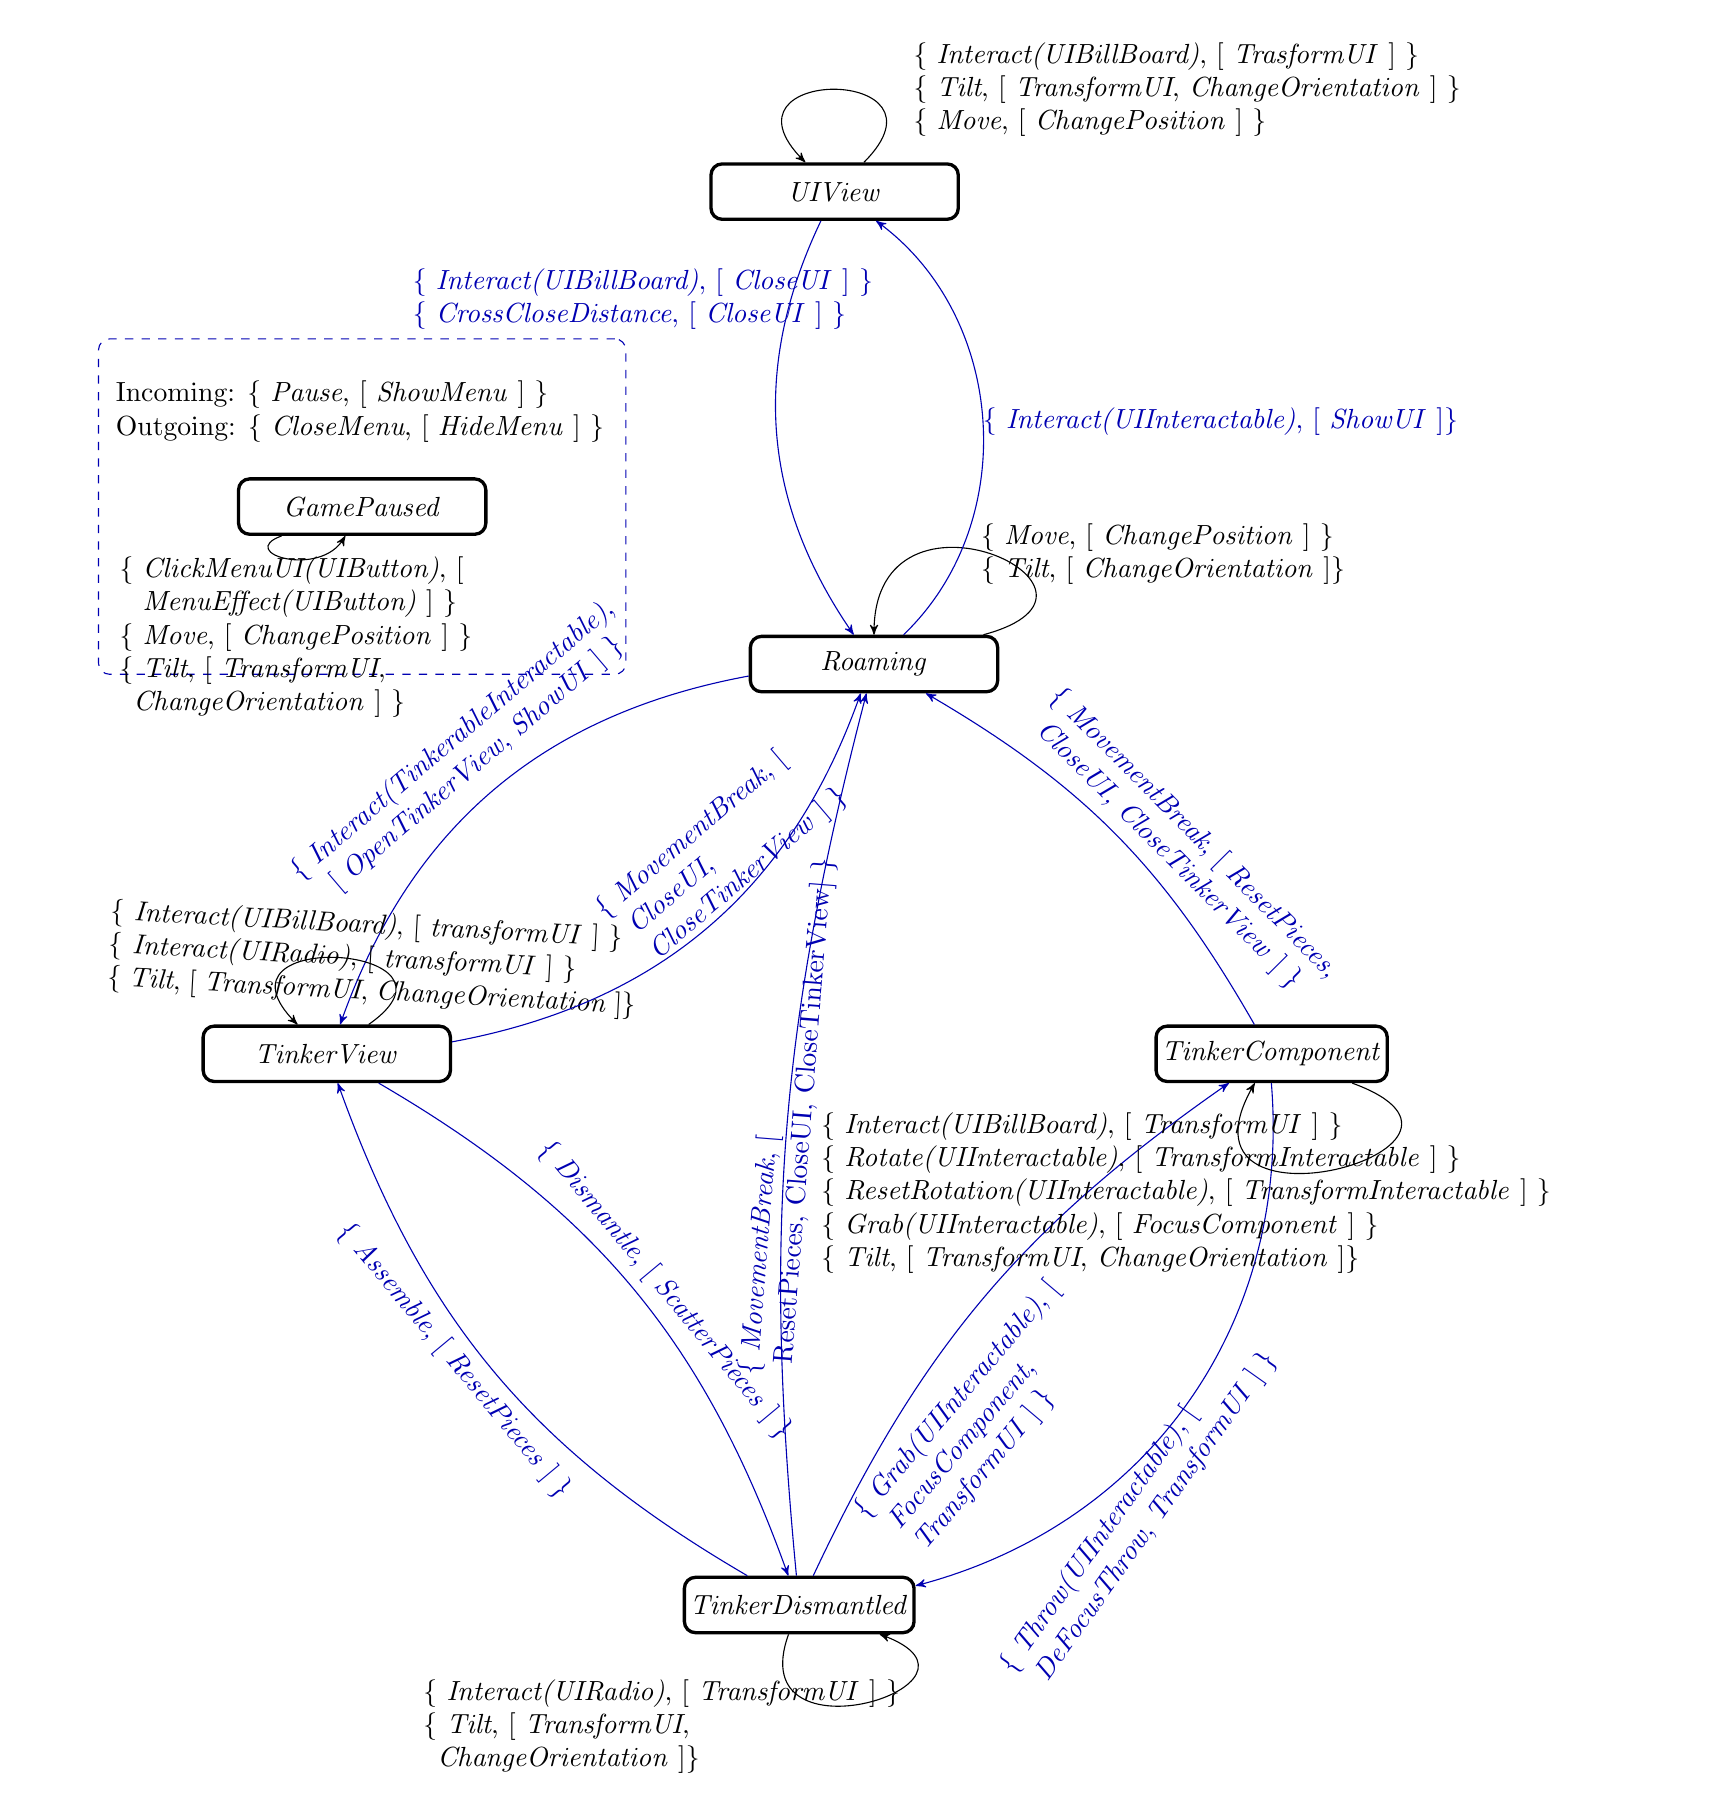
\begin{tikzpicture}[->,>=stealth']
        \node[state,
          text width=3cm,
          anchor=center] (ROAMING)
          {\textit{Roaming}};

        \node[state,
          text width=3cm,
          yshift=2cm,
          left of=ROAMING,
          node distance=6.5cm] 
          (GAMEPAUSED) {\textit{GamePaused}};

        \node[draw, rectangle, rounded corners, dashed, anchor=center,
          fit={(GAMEPAUSED)}, inner sep=50pt, color=blue!70!black] 
          (GAMEPAUSEDFRAME) {};
        \node[above left of=GAMEPAUSED, node distance=1cm, anchor=center, 
          yshift=0.5cm, xshift=0.3cm] {
            \parbox{7.2cm}{\begin{itemize}[noitemsep, topsep=0pt]
              \item[] Incoming: \{ \textit{Pause}, [ \textit{ShowMenu} ] \}
              \item[] Outgoing: \{ \textit{CloseMenu}, [ \textit{HideMenu} ] \}
            \end{itemize}}
        };
        
        \node[state,
          text width=3cm,
          yshift=4cm,
          right of=GAMEPAUSED,
          node distance=6cm,
          anchor=center] (UIVIEW)
          {\textit{UIView}};
       
        \node[state,
          below left of=ROAMING,
          node distance=7cm,
          xshift=-2cm,
          anchor=center,
          text width=3cm] (TINKERVIEW) 
          {\textit{TinkerView}};

        \node[state,
          right of=TINKERVIEW,
          node distance=6cm,
          yshift=-7cm,
          anchor=center] (TINKERDISMANTLED) 
          {\textit{TinkerDismantled}};

        \node[state,
          right of=TINKERVIEW,
          node distance=12cm,
          anchor=center] (TINKERCOMPONENT) 
          {\textit{TinkerComponent}};

        % draw the paths and and print some Text below/above the graph
        \path (ROAMING) edge[loop above, in=90, out=15, looseness=4] 
          node[anchor=center, xshift=2cm]{
            \parbox{6cm}{\begin{itemize}[noitemsep, topsep=0pt]
              \item[] \{ \textit{Move}, [ \textit{ChangePosition} ] \}
              \item[] \{ \textit{Tilt}, [ \textit{ChangeOrientation} ]\}
            \end{itemize}}
          } (ROAMING)
        (ROAMING) edge[bend right=50, above left, color=blue!70!black] 
        node[anchor=above,right,xshift=-1cm] {
          \parbox{7cm}{\begin{itemize}[noitemsep, topsep=0pt]
            \item[] \{ \textit{Interact(UIInteractable)}, [ \textit{ShowUI} ]\}
          \end{itemize}}
        } (UIVIEW)
        (UIVIEW) edge[loop above, in=135, out=45, looseness=6] node[anchor=below,right] {
          \parbox{8cm}{\begin{itemize}[noitemsep, topsep=0pt]
            \item[] \{ \textit{Interact(UIBillBoard)}, [ \textit{TrasformUI} ] \}
            \item[] \{ \textit{Tilt}, [ \textit{TransformUI}, \textit{ChangeOrientation} ] \}
            \item[] \{ \textit{Move}, [ \textit{ChangePosition} ] \}
          \end{itemize}}
        } (UIVIEW)
        (UIVIEW) edge[bend right=30, below left, color=blue!70!black] node[anchor=center, yshift=1.7cm, xshift=-2cm] {
          \parbox{7cm}{\begin{itemize}[noitemsep, topsep=0pt]
            \item[] \{ \textit{Interact(UIBillBoard)}, [ \textit{CloseUI} ] \}
            \item[] \{ \textit{CrossCloseDistance}, [ \textit{CloseUI} ] \}
          \end{itemize}}
        } (ROAMING)
        (ROAMING) edge[bend right=30, below left, color=blue!70!black] node[sloped, anchor=center, yshift=0.6cm] {
          \parbox{7cm}{\begin{itemize}[noitemsep, topsep=0pt]
            \item[] \{ \textit{Interact(TinkerableInteractable)}, 
            \item[] \hspace{0.5em} [ \textit{OpenTinkerView}, \textit{ShowUI} ] \}
          \end{itemize}}
        } (TINKERVIEW)
        (TINKERVIEW) edge[loop left, in=135, out=35, looseness=5] node[sloped, anchor=center] {
          \parbox{7.6cm}{\begin{itemize}[noitemsep, topsep=0pt]
            \item[] \{ \textit{Interact(UIBillBoard)}, [ \textit{transformUI} ] \}
            \item[] \{ \textit{Interact(UIRadio)}, [ \textit{transformUI} ] \}
            \item[] \{ \textit{Tilt}, [ \textit{TransformUI}, \textit{ChangeOrientation} ]\}
          \end{itemize}}
        } (TINKERVIEW)
        (TINKERVIEW) edge[bend right=30, below right, color=blue!70!black] 
          node[sloped, anchor=center,xshift=1.2cm, yshift=0.6cm] {
          \parbox{6cm}{\begin{itemize}[noitemsep, topsep=0pt]
            \item[] \{ \textit{MovementBreak}, [ 
            \item[] \hspace{0.5em}\textit{CloseUI}, 
            \item[] \hspace{0.5em}\textit{CloseTinkerView} ] \}
          \end{itemize}}
        } (ROAMING)
        (TINKERVIEW) edge[bend left=20, below, color=blue!70!black] 
          node[sloped, anchor=center, yshift=0.3cm, xshift=0.5cm] {
            \parbox{7cm}{\begin{itemize}[noitemsep, topsep=0pt]
              \item[] \{ \textit{Dismantle}, [ \textit{ScatterPieces} ] \}
            \end{itemize}}
          } (TINKERDISMANTLED)
        (TINKERDISMANTLED) edge[bend left=20, below, color=blue!70!black] 
          node[sloped, anchor=center, yshift=-0.3cm] {
            \parbox{7cm}{\begin{itemize}[noitemsep, topsep=0pt]
              \item[] \{ \textit{Assemble}, [ \textit{ResetPieces} ] \}
            \end{itemize}}
          } (TINKERVIEW)
        (TINKERDISMANTLED) edge[loop below, in=340, out=250, looseness=4] 
          node[anchor=center, xshift=-3cm, yshift=-0.3cm] {
            \parbox{7cm}{\begin{itemize}[noitemsep, topsep=0pt]
              \item[] \{ \textit{Interact(UIRadio)}, [ \textit{TransformUI} ] \}
              \item[] \{ \textit{Tilt}, [ \textit{TransformUI}, 
              \item[] \hspace{0.5em}\textit{ChangeOrientation} ]\}
            \end{itemize}}
          } (TINKERDISMANTLED)
        (TINKERDISMANTLED) edge[bend left=10, right, color=blue!70!black]
          node[sloped, anchor=center] {
            \parbox{8cm}{\begin{itemize}[noitemsep, topsep=0pt]
              \item[] \{ \textit{MovementBreak}, [
              \item[] \hspace{0.5em}ResetPieces, CloseUI, CloseTinkerView] \}
            \end{itemize}}
          } (ROAMING)
        (TINKERDISMANTLED) edge[bend left=15, below right, color=blue!70!black] 
          node[sloped, anchor=center, yshift=-1cm] {
            \parbox{8cm}{\begin{itemize}[noitemsep, topsep=0pt]
              \item[] \{ \textit{Grab(UIInteractable)}, [ 
              \item[] \hspace{0.5em}\textit{FocusComponent}, 
              \item[] \hspace{0.5em}\textit{TransformUI} ] \}
            \end{itemize}}
          } (TINKERCOMPONENT)
        (TINKERCOMPONENT) edge[bend left=40, below, color=blue!70!black]
          node[sloped, anchor=center, yshift=-0.3cm, xshift=-1cm] {
            \parbox{8cm}{\begin{itemize}[noitemsep, topsep=0pt]
              \item[] \{ \textit{Throw(UIInteractable)}, [ 
              \item[] \hspace{0.5em}\textit{DeFocusThrow}, \textit{TransformUI} ] \}
            \end{itemize}}
          } (TINKERDISMANTLED)
        (TINKERCOMPONENT) edge[loop below, in=240, out=340, looseness=5]
          node[anchor=center, yshift=-0.3cm, xshift=-1.4cm] {
            \parbox{12cm}{\begin{itemize}[topsep=0pt, noitemsep]
              \item[] \{ \textit{Interact(UIBillBoard)}, [ \textit{TransformUI} ] \}
              \item[] \{ \textit{Rotate(UIInteractable)}, [ \textit{TransformInteractable} ] \}
              \item[] \{ \textit{ResetRotation(UIInteractable)}, [ \textit{TransformInteractable} ] \}
              \item[] \{ \textit{Grab(UIInteractable)}, [ \textit{FocusComponent} ] \}
              \item[] \{ \textit{Tilt}, [ \textit{TransformUI}, \textit{ChangeOrientation} ]\}
            \end{itemize}}
          } (TINKERCOMPONENT)
        (TINKERCOMPONENT) edge[bend right=15, above, color=blue!70!black]
          node[sloped, anchor=center, xshift=3.3cm,yshift=0.5cm] {
            \parbox{12cm}{\begin{itemize}[noitemsep, topsep=0pt]
              \item[] \{ \textit{MovementBreak}, [ \textit{ResetPieces, 
              \item[] \hspace{0.5em}CloseUI, CloseTinkerView} ] \}
            \end{itemize}}
          } (ROAMING)
        (GAMEPAUSED) edge[loop below, out=200, in=240, looseness=2] 
          node[anchor=center, yshift=-1cm] {
            \parbox{6cm}{\begin{itemize}[noitemsep, topsep=0pt]
              \item[] \{ \textit{ClickMenuUI(UIButton)}, [ 
              \item[] \hspace{0.5em} \textit{MenuEffect(UIButton)} ] \}
              \item[] \{ \textit{Move}, [ \textit{ChangePosition} ] \}
              \item[] \{ \textit{Tilt}, [ \textit{TransformUI}, 
              \item[] \hspace{0.5em}\textit{ChangeOrientation} ] \}
            \end{itemize}}
          } (GAMEPAUSED);
      \end{tikzpicture}\end{adjustbox}
      \vspace{3pt}
      \hrule
      \vspace{3pt}
      \caption{Rappresentazione Diagramma a Stati dell'interazione dell'utente, collegando tutte le \textit{Action} e \textit{Effects} citati nelle tabelle a pagina precedente. 
        I collegamenti con lo stato \textit{GamePaused} sono stati omessi}
      \end{mdframed}
    \end{figure}
    \FloatBarrier
    \needspace{3\baselineskip}
    \footnotetext[9]{Questi bottoni permettono di trasformare la \textit{UIBillboard} per mostrare il contenuto relativo al singolo componente}
    \footnotetext[10]{tasto di chiusura}
    \footnotetext[11]{nel caso sei nello stato \textit{UIView}, l'\textit{Interact(TinkerableInteractable)} prima esegue gli effetti associati alla classe base
      \textit{UIInteractable}, ovvero la chiusura del \textit{UIInteractable} precedentemente aperto.}
    \setcounter{footnote}{11} 
    \subsection{Storyboards}
    da fare
    \section{Feedback e Cues}\label{vr:feedback}
    I vari feedback sensoriali da implementare nella simulazione derivano dalla interazione tra utente e \textit{Interactable}s, e tra utente e Ambiente.
    \subsection{Video}
    \begin{table}[h]
      \centering
      \begin{tabular}{@{} p{0.3\textwidth} p{0.7\textwidth} @{}}
        \toprule
        \textbf{Stimolo} & \textbf{Risposta} \\
        \midrule
        \textit{Move}, \textit{Tilt} & Spostamento all'interno dell'ambiente di gioco. \\
        \textit{Interact} & Apparizione o Trasformazione degli Elementi UI Spaziali (\textit{UIBillBoard}) o posizionamento del \textit{TinkerableInteractable}. \\
        \textit{Dismantle}, \textit{Assemble} & Rispettivamente Decomposizione "esplosiva" e Reset di tutti i componenti del \textit{TinkerableInteractable}. \\
        \textit{Grab} & Posizionamento del \textit{UIInteractable} selezionato in una posizione predefinita antestante alla camera (Desktop) oppure su un ancora posizionata sulla 
          mano che ha compiuto l'azione (HMD VR) \\
        \textit{Rotate}, \textit{ResetRotation} & Cambiamento dell'orientamento del \textit{UIInteractable} fissato nella posizione di ancoraggio (Stato \textit{TinkerComponent}) \\
        \textit{Pause}, \textit{CloseMenu} & Rispettivamente Apparizione e Scomparsa elementi UI del menu di pausa. \\
        Interazione con varie UI Spazializzate & Trasformazione del contenuto visivo UI in risposta all'azione specifica compiuta dall'utente, quali
          \begin{itemize}[noitemsep, topsep=0pt]
            \item Scomparsa \textit{UIBillBoard} di un \textit{UIInteractable} in seguito alla pressione del tasto di chiusura o allontanamento da parte dell'utente
            \item Scambio dei pulsanti di menu di pausa mostrati (\textit{MenuEffect}) in seguito alla pressione di uno \textit{UIButton} (Stato \textit{GamePaused})
            \item Riproduzione del contenuto multimediale (audio associato ad un paragrafo della \textit{UIBillBoard} o animazione associata ad un \textit{SequenceInteractable}, i cui 
              bottoni per controllare la riproduzione si trovano nella \textit{UIBillBoard} associata)
          \end{itemize} \\
        Chiusura Sessione di interazione con \textit{TinkerableInteractable} o \textit{UIInteractable} & Scomparsa elemento \textit{UIBillboard} e riposizionamento posizione originale
          del \textit{TinkerableInteractable} \\
        \bottomrule
      \end{tabular}
    \end{table}
    \FloatBarrier
    \needspace{0.3\paperheight}
    \subsection{Audio}
    \begin{table}[h]
      \centering
      \begin{tabular}{@{} p{0.3\textwidth} p{0.7\textwidth} @{}}
        \toprule
        \textbf{Stimolo} & \textbf{Risposta} \\
        \midrule
        interazione con varie UI & Sound Effect pressione pulsante \\
        \textit{Dismantle}, \textit{Assemble} & Sound Effect decomposizione e riassemblaggio oggetto. Ciascun oggetto deve possedere un sound effect che richiami i materiali di cui 
          l'oggetto \`e costituito (per lo pi\`u oggetti metallici quali firearms) \\
        \textit{Move} & Sound Effect associato alla camminata dell'utente, il quale pu\`o variare a seconda del pavimento su cui si sta camminando. Possibili variazioni possono essere
          \begin{itemize}[noitemsep, topsep=0pt]
            \item Pavimento di Mattoni
            \item Pavimento di Legno
            \item Scalinata
          \end{itemize} \\
        \textit{Grab}, \textit{Throw} & Sound Effect associati alla presa e lancio di un \textit{UIInteractable} \\
        \bottomrule
      \end{tabular}
    \end{table}
    \FloatBarrier
    \needspace{3\baselineskip}
    \subsection{Aptico}
    \begin{table}[h]
      \centering
      \begin{tabular}{@{} p{0.3\textwidth} p{0.7\textwidth} @{}}
        \toprule
        \textbf{Stimolo} & \textbf{Risposta} \\
        \midrule
        Riproduzione di Un suono impulsivo, eg. esplosione\footnotemark{} & vibrazione degli XR Hand Controller (applicabile in modalit\`a HMD VR) \\
        \textit{Throw} & vibrazione dell'XR Hand Controller che ha lanciato il \textit{UIInteractable} \\
        \bottomrule
      \end{tabular}
    \end{table}
    \footnotetext{Immagina una bomba un sul campo di battaglia miniaturizzato in Sala 7 del museo (digramma)}
    \FloatBarrier
    \section{Audio}\label{vr:audio}
    Al fine di incrementare il senso di immersione della simulazione, assets audio slegati dal feedback sulle azioni utente (Vedi sezione \ref{vr:feedback}). In particolare,
    una BGMs per l'esplorazione del museo devono presentare alcune tra le seguenti caratteristiche
    \begin{itemize}[noitemsep, topsep=0pt]
      \item \textbf{Somber Elegance} Arrangiamento basato su corde (violino) e melodia con pianoforte, che riflette la seriet\`a della guerra, con occasionali strumenti in ottone come
        la Tromba barocca per aggiungere profondit\`a e senso di discovery.
      \item \textbf{Marcia Militare} Composizione dal tempo di 60 bpm basato su trumenti come trombone e fanfara. Per maggiori informazioni, 
        \href{https://it.wikipedia.org/wiki/Marcia_(musica)#Struttura_e_caratteristiche}{Wikipedia}
      \item \textbf{Echo del passato} Suoni distanti distanti di guerra, come urla, esplosioni, proiettili, utilizzati in zone pertinenti come il Corridoio Ovest del Piano interrato, 
        il quale, Nel museo di riferimento, riproduce una trincea con audio spazializzato.
      \item \textbf{Richiami alle Musiche Corali} tipiche del periodo della prima guerra mondiale, come hymns o folk tunes.
    \end{itemize}
    Circa la natura dell audio, si specifica che
    \begin{itemize}[topsep=0pt, noitemsep]
      \item Tutte le BGM sono Audio 2D Monoaurale, la cui scelta, con Fade in e Fade out, dipende unicamente dalla sala in cui l'utente si trova e dallo stato della 
        simulazione (Tabella \ref{vr:states})
      \item Tutti i Sound Effect, provenienti da Azioni Utente, comprese le interazioni con UI, sono spazializzati.
    \end{itemize}
  \section{Sistemi}
  Dalle caratteristiche dettagliate a Paragrafo \ref{vr:ux}, riconosciamo essenzialmente due sistemi principali atti ad implementare l'interazione con l'utente, escluso il Character
  Controller dell'\textit{Player Pawn} stesso:
  \begin{itemize}[noitemsep, topsep=0pt]
    \item \textbf{\textit{TextSynthesiser}} Sistema Responsabile di Prendere in input una specifica di testo da mostrare su \textit{UIBillboard}, La width e height massime con cui 
      renderizzare il contenuto, eventuale trasformazione di rotazione/traslazione, al fine di preparare la \textit{UIBillBoard} per la visualizzazione.
    \item \textbf{\textit{Interactables System}} Sistema Responsabile della gestione degli eventi diretti a ciascun Interactable 
  \end{itemize}
  Partendo dalla gerarchia degli \textit{Interactable}s, di seguito \`e mostrato uno UML Class Diagram rappresentante, ad alto livello di astrazione, le funzionalit\`a che ciascuna 
  tipologia di \textit{Interactable} mette a disposizione:
  \begin{figure}[h]
    \centering
    \begin{adjustbox}{max width=0.9\paperwidth, frame=1pt 4pt, center}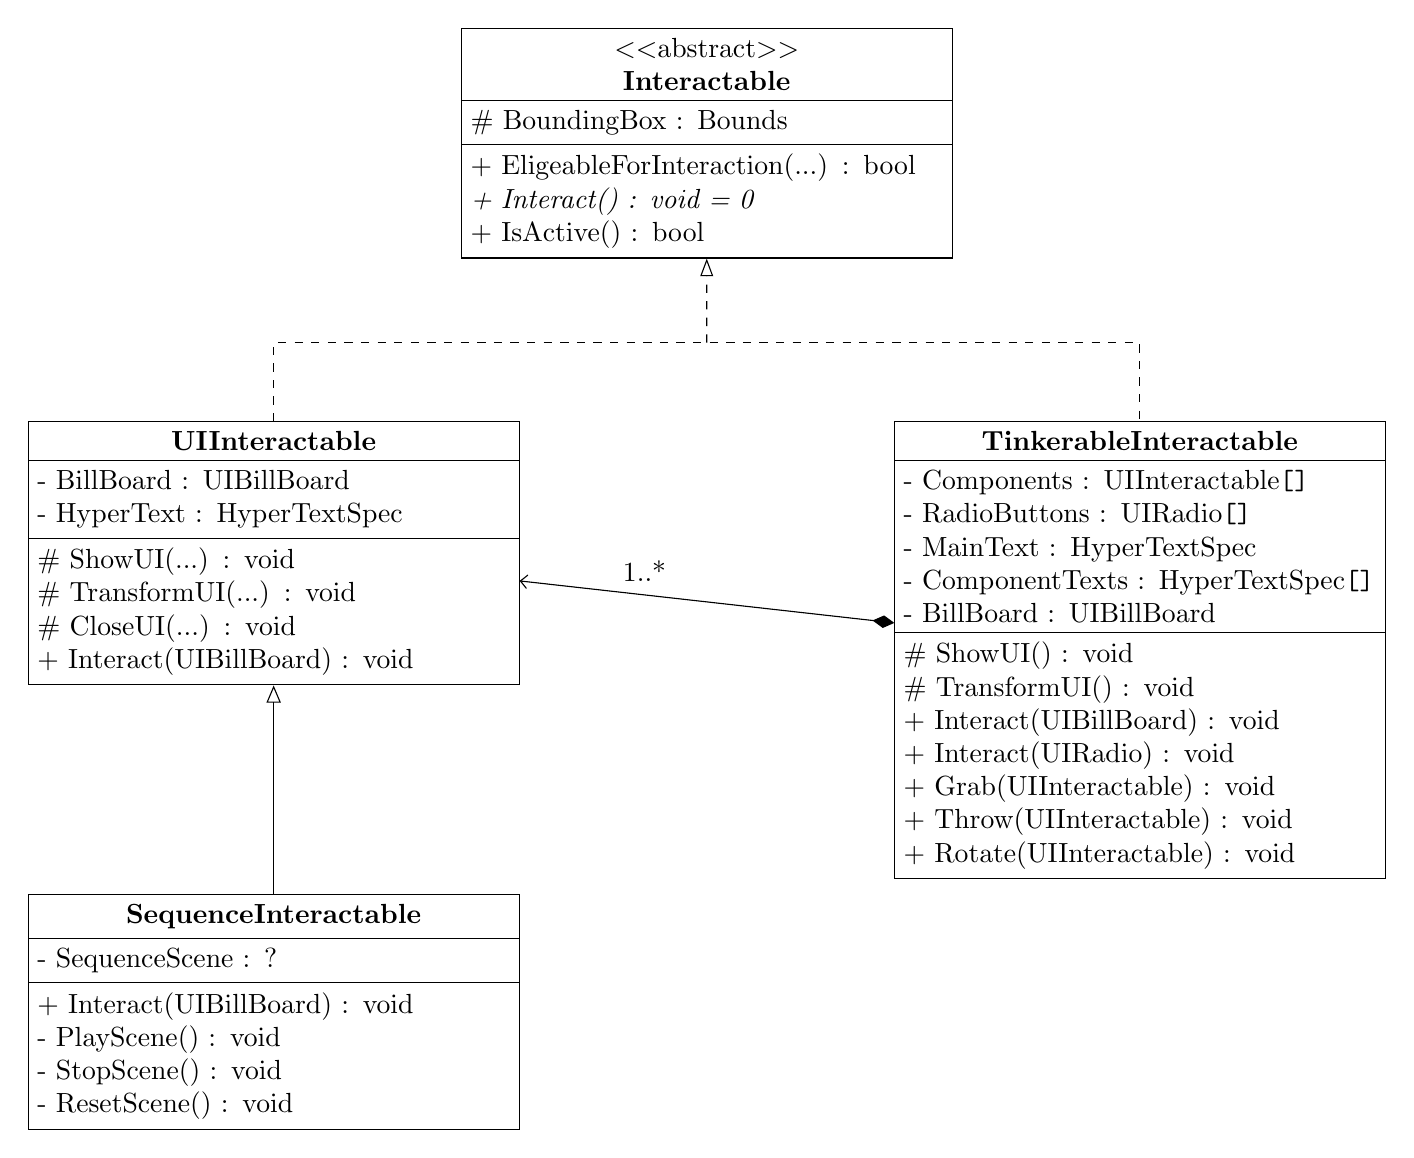
\begin{tikzpicture}
      \renewcommand{\umltextcolor}{black}
      \renewcommand{\umlfillcolor}{white}
      \renewcommand{\umldrawcolor}{black}
      \begin{abstractclass}[text width=6cm]{Interactable}{5.5,0}
        \attribute{\# BoundingBox : Bounds}
        \operation{+ EligeableForInteraction(...) : bool}
        \operation[0]{+ Interact() : void = 0}
        \operation{+ IsActive() : bool}
      \end{abstractclass}

      \begin{class}[text width=6cm]{UIInteractable}{0,-5}
        %\implement{Interactable}
        \attribute{- BillBoard : UIBillBoard}
        \attribute{- HyperText : HyperTextSpec}
        \operation{\# ShowUI(...) : void}
        \operation{\# TransformUI(...) : void}
        \operation{\# CloseUI(...) : void}
        \operation{+ Interact(UIBillBoard) : void}
      \end{class}

      \begin{class}[text width=6cm]{SequenceInteractable}{0, -11}
        \inherit{UIInteractable}
        \attribute{- SequenceScene : ?}
        \operation{+ Interact(UIBillBoard) : void}
        \operation{- PlayScene() : void}
        \operation{- StopScene() : void}
        \operation{- ResetScene() : void}
      \end{class}

      \begin{class}[text width=6cm]{TinkerableInteractable}{11, -5}
        %\implement{Interactable}
        \attribute{- Components : UIInteractable\texttt{[]}}
        \attribute{- RadioButtons : UIRadio\texttt{[]}}
        \attribute{- MainText : HyperTextSpec}
        \attribute{- ComponentTexts : HyperTextSpec\texttt{[]}}
        \attribute{- BillBoard : UIBillBoard}
        \operation{\# ShowUI() : void}
        \operation{\# TransformUI() : void}
        \operation{+ Interact(UIBillBoard) : void}
        \operation{+ Interact(UIRadio) : void}
        \operation{+ Grab(UIInteractable) : void}
        \operation{+ Throw(UIInteractable) : void}
        \operation{+ Rotate(UIInteractable) : void}
      \end{class}
      \composition{TinkerableInteractable}{}{1..*}{UIInteractable}

      \draw[umlcd style dashed line](UIInteractable.north) -- ++(0, 1) coordinate(left) 
        -- ++(5.5cm, 0) coordinate(mid) 
        -- (TinkerableInteractable.north|-mid) coordinate(midright) 
        -- (TinkerableInteractable.north);

      \draw[umlcd style dashed line, -{Triangle[open,scale=1.5, angle=40:4.5]}] (mid) 
        -- (Interactable.south);
    \end{tikzpicture}\end{adjustbox}
  \end{figure}
  \FloatBarrier
  Passo all'analisi preliminare del Sistema \textit{TextSyntesiser}.\\
  Unity possiede \href{https://docs.unity3d.com/6000.0/Documentation/Manual/UIToolkits.html}{tre modalit\`a} per definire elementi UI all'interno del runtime o dell'editor stesso
  \begin{itemize}[leftmargin=33mm, topsep=0pt, noitemsep]
    \item[\textbf{UI Toolkit}] Definizione di una UI a partire da dei documenti di contenuto e di stile, simile all'approccio web HTML + CSS
    \item[\textbf{uGUI package}] Ogni elemento UI (testo, slider, ...) \`e un gameObject. Il testo di cui si parla \`e 
      \href{https://docs.unity3d.com/Packages/com.unity.ugui@2.0/manual/TextMeshPro/RichTextSupportedTags.html}{Rich Text}
    \item[\textbf{IMGUI}] Sistema GUI code-driven, dove l'interfaccia \`e specificata interamente in \texttt{C\#}
  \end{itemize}
  Unity consiglia di utilizzare UI Toolkit per estensioni dello Unity Editor, uGUI per Runtime UI, e IMGUI per interfacce di debug. Dunque il nostro sistema utilizzar\`a \textbf{uGUI}.\par
  Il flusso ad alto livello \`e il seguente.\\
%  \begin{egdlisting}[style=sharpc]
  \begin{minipage}[t]{0.48\textwidth}
    \vspace{0pt}
    \begin{adjustbox}{left, outer, frame=1pt 2pt, max width=\textwidth}\begin{lstlisting}[style=sharpc]
(UIStage.cs)
public void OnCursorInput() {
  - Quando il componente UI riceve input 
    dal mouse (evento da Quad Display)
  - Dati posizione click, mouse button
  - Determinare Elemento UI Premuto
  - Dispatch Evento all'Elemento UI
}

(UIDisplayScene.cs)
public void Update() {
  - Dato Mouse Position, ScreenPointToRay 
    Dalla MainCamera per determinare se 
    Raycast colpisce pannello UI
  - Dispatch Cursor Input alla UI
}
    \end{lstlisting}\end{adjustbox}
  \end{minipage}
%  \end{egdlisting}
  \begin{minipage}[t]{0.48\textwidth}
    \vspace{0pt}
    \begin{itemize}[topsep=0pt, noitemsep]
      \item \texttt{Canvas} con \texttt{RenderMode: World Space}
      \item \texttt{Graphics Raycaster} OFF, affinch\`e non venga inviato un evento
        quando l'oggetto UI stesso, nascosto dalla MainCamera perch\`e in un layer diverso, viene toccato dal mouse
      \item Usare una capture camera con \texttt{Orthographic Projection} per renderizzare l'elemento UI su una texture
        \texttt{Render Target}
      \item Applicare ad un Quad, o mesh arbitraria, la texture prodotta, per mostrare l'UI in modo spazializzato
    \end{itemize}
    \href{https://www.youtube.com/watch?v=dPdmJ0RDLSI}{Video di riferimento}
  \end{minipage}
  \FloatBarrier
  Il contenuto delle interfacce grafiche mostrate tramite gli \textit{UIBillBoard}s hanno la seguente struttura (Esempio in Paragrafo \ref{vr:ui})
  \begin{itemize}[topsep=0pt, noitemsep]
    \item \textbf{Titolo Principale}, tipicamente il nome dell'oggetto ispezionato. Bianco, bold, font size leggermente superiore al corpus del testo
    \item \textbf{Paragrafi di testo}, ciascuno con Titolo bold, corpus espandibile/comprimibile composto da rich text, play button per riprodurre una versione audio del paragrafo
    \item Larghezza della BillBoard prefissata, e se un periodo la supera, la parola che supera i limite orizzontale viene sillabata e spostata a rigo successivo
    \item Altezza della BillBoard prefissata, e se la totalit\`a dei paragrafi, con corpus mostrato o no, la superano, allora viene gestito l'overflow testuale con l'inserimento di 
      uno slider
  \end{itemize}
  Ci\`o che cambia \`e solamente il contenuto. Dunque, si \`e pensato di realizzare uno script che prende in input una descrizione dei paragrafi che compongono il contenuto
  della \textit{UIBillBoard}, e ne istanzia i necessari gameObjects\footnote{utilizzando uGUI 2.0} per concretizzare l'interfaccia grafica. Tale descrizione pu\`o essere data attraverso
  un file \href{https://toml.io/en/v1.0.0}{TOML}\footnote{Soggetto a cambiamento. Nota come non si supporta inserimento di immagini.}
  \begin{lstlisting}[style=toml]
[header]
max_width = 2 # in metri
max_height = 3 # in metri
title = "Fiat-Revelli Mod. 1914"

[[body.paragraphs]] # array, elemento 0
# titolo del paragrafo puo non esserci, in tal caso il corpus non si comprime
# path relativa alla posizione del file TOML dell'audio per paragrafo
audio = "../Audio/Fiat-Revelli-1914/par0.wav"
# rich text corpus. Se l'ultimo carattere di riga e \, allora escape newline
corpus = """/*{\color{gray60}\texttt{\# newline come primo carattere non viene contato (ultimo si)}}*/
La <b>Fiat-Revelli Mod.1914</b> è stata una mitragliatrice media, \
adottata dal Regio Esercito Italiano nella prima guerra Mondiale."""

[[body.paragraphs]]
title = "Storia"
audio = "../Audio/Fiat-Revelli-1914/par1.wav"
corpus = """
Il progetto dell'arma risale al 1910 eccetera."""
  \end{lstlisting}
Sapendo che Unity 6 utilizza \texttt{C\#} 9.0, un TOML parser compatibile \`e disponibile al \href{https://github.com/dezhidki/Tommy}{Seguente Link}.
  \section{UI}\label{vr:ui}
  \FloatBarrier
  Data la natura illustrativa della simulazione, non sono presenti UI di tipo \textit{Non-Diegetic} o \textit{Meta}. Sono invece presenti
  \begin{itemize}[topsep=0pt, noitemsep]
    \item \textit{Diegetic} UI, in quanto su un \textit{Interactable} marcato come selezionabile compare un outline
    \item \textit{Spatial} Sottoforma di \textit{UIBillBoard} sopracitate
  \end{itemize}
  \`E Mostrata in Figura \ref{vr:ui:figinteraction} un esempio di dinamica di interazione con un \textit{UIInteractable}.
  \begin{figure}[t]
    \begin{mdframed}[
      linecolor=black,
      linewidth=1pt,
      innertopmargin=6pt,
      innerbottommargin=6pt,
      innerleftmargin=6pt,
      innerrightmargin=6pt
    ]
        \begin{subfigure}[b]{\textwidth}
        \includegraphics[width=\textwidth]{UI_eligeable_for_selection.png}\\
        \end{subfigure}
        \begin{subfigure}[b]{\textwidth}
        \includegraphics[width=\textwidth]{UI_UIView_State_with_another_eligeable_for_selection.png}
        \end{subfigure}
      \vspace{3pt}
      \hrule
      \vspace{3pt}
      \caption{In Alto, \`e mostrato un esempio di \textit{UIInteractable} che soddisfa tutti i requisiti per poter essere selezionato, dunque viene mostrato un outline. Una volta che 
        l'azione \textit{Interact(UIInteractable)} \`e stata compiuta, il colore della outline cambia (e diventa visibile da oltre i muri), e viene renderizzato un 
        \textit{UIBillBoard}, come mostrato nell'immagine in basso\protect\footnotemark. 
        Si nota come se un altro \textit{Interactable} \`e selezionabile nello stato \textit{UIView}, allora la sua outline viene mostrata.}
      \label{vr:ui:figinteraction}
    \end{mdframed}
  \end{figure}
  \footnotetext{Nota come sono assenti i play buttons per ogni paragrafo. L'immagine \`e a puro scopo illustrativo.}
  \FloatBarrier
  \section{Assets}
  \subsection{References}
  Di seguito sono riportate immagini di riferimento per props presenti nei vari ambienti. Per immagini ritraenti gli ambienti del museo di riferimento, consultare 
  sottoparagrafo \ref{vr:planimetria}
  \FloatBarrier
  Inoltre, in quanto si vogliono approfondire anche alcuni aspetti sulla tecnologia bellica dell'alba del XX Secolo, di seguito link utili di riferimento
  \renewcommand{\arraystretch}{1.5} % aumenta spaziatura tra righe per non confondere paragrafi multilinea
  \begin{table}[h]\label{vr:weapons}
    \centering
    \begin{tabular}{@{} p{0.35\textwidth} p{0.65\textwidth} @{}}
      \toprule
      \textbf{Categoria Arma da Fuoco} & \textbf{Elenco di riferimenti ipertestuali} \\
      \midrule
      \href{https://it.wikipedia.org/wiki/Pistola}{Pistole} 
        & \href{https://it.wikipedia.org/wiki/Glisenti_Modello_1910}{Glisenti Modello 1910} | \href{https://it.wikipedia.org/wiki/Brixia_Mod._1913}{Brixia Mod. 1913} | 
          \href{https://it.wikipedia.org/wiki/Bodeo_Mod._1889}{Bodeo Mod. 1889} | \href{https://it.wikipedia.org/wiki/Beretta_M15}{Beretta M15} | 
          \href{https://it.wikipedia.org/wiki/Beretta_M17}{Beretta M17} \\
      \href{https://it.wikipedia.org/wiki/Fucile}{Fucili} e \href{https://it.wikipedia.org/wiki/Carabina}{Carabine} 
        & \href{https://it.wikipedia.org/wiki/Carcano_Mod._91}{Carcano Mod. 91} | \href{https://it.wikipedia.org/wiki/Vetterli-Vitali_Mod._1870/87}{Vetterli-Vitali Mod. 1870/86} |
          \href{https://it.wikipedia.org/wiki/Vetterli-Vitali_Mod._1870/87/16}{Vetterli-Vitali Mod. 1870/86/16} \\
      \href{https://it.wikipedia.org/wiki/Pistola_mitragliatrice}{Pistole Mitragliatrici} e \href{https://it.wikipedia.org/wiki/Mitra_(arma)}{Mitra}
        & \href{https://it.wikipedia.org/wiki/Beretta_MAB_18}{Beretta MAB 18} | \href{https://it.wikipedia.org/wiki/Villar_Perosa_(arma)}{Villar Perosa} | 
          \href{https://it.wikipedia.org/wiki/OVP}{Fiat OVP} \\
      \href{https://it.wikipedia.org/wiki/Mitragliatrice}{Mitragliatrici} e armi pesanti 
        & \href{https://it.wikipedia.org/wiki/Fiat-Revelli_Mod._1914}{Fiat-Revelli Mod. 1914} | \href{https://it.wikipedia.org/wiki/Perino_Mod._1908}{Perino Mod. 1908} |
          \href{https://it.wikipedia.org/wiki/SIA_Mod._1918}{SIA Mod. 1918} | \href{https://en.wikipedia.org/wiki/Gardner_gun}{Gardner M1886} | 
          \href{https://royalarmouries.org/collection/object/object-15528}{Nordenfelt Mod. 1884} | 
          \href{https://www.vhu.cz/en/exhibit/18-french-flamethrower-schilt-no-3-bis-c-1917/}{Lanciafiamme Schilt 1, 2, 3bis}\footnotemark, 
          \href{https://www.vhu.cz/en/exhibit/17-italsky-maly-plamenomet-d-l-f-1918/}{Lanciafiamme DLF} | 
          \href{https://www.youtube.com/watch?v=HWPtTujOITM}{Lanciafiamme Hersent-Thiriont} | Apparato a Twin-Tank \\
      \href{https://it.wikipedia.org/wiki/Bomba_a_mano}{Bombe a mano} e da fucile offensive, difensive e incendiarie 
        & \href{https://it.wikipedia.org/wiki/Aasen_tipo_A2}{Aasen tipo A2} |
          \href{https://it.wikipedia.org/wiki/Aasen_tipo_C}{Aasen tipo C} |
          \href{https://it.wikipedia.org/wiki/Aasen_da_fucile}{Aasen da fucile} |
          \href{https://it.wikipedia.org/wiki/Baldari_(granata)}{Baldari} |
          \href{https://it.wikipedia.org/wiki/Excelsior-Th%C3%A9venot_P2}{Ballerina} |
          \href{https://it.wikipedia.org/wiki/Benaglia_(bomba_da_fucile)}{Benaglia} |
          \href{https://it.wikipedia.org/wiki/Bertone_(bomba_da_fucile)}{Bertone} |
          \href{https://it.wikipedia.org/wiki/Besozzi_(granata)}{Besozzi} |
          \href{https://it.wikipedia.org/wiki/BPD_(granata)}{BPD} |
          \href{https://it.wikipedia.org/wiki/Carasco_(granata)}{Carasco} |
          \href{https://www.talpo.it/granata-carbone.html}{Carbone} |
          \href{https://web.archive.org/web/20160304190108/http://www.talpo.it/files/istruzioni_caricamento_lenticolare_m14.pdf}{Lenticolare Mod. 1914} |
          \href{https://www.talpo.it/lenticolare-minucciani.html}{Lenticolare Minucciani} |
          \href{https://www.talpo.it/petardo-stobi.html}{Petardo Stobi} |
          \href{https://web.archive.org/web/20120621113432/http://www.talpo.it/petardo_thevenot.html}{Petardo Thévenot} |
          \href{https://it.wikipedia.org/wiki/SIPE}{SIPE} |
          \href{https://it.wikipedia.org/wiki/Spaccamela_(granata)}{Spaccamela} |
          % \href{https://www.talpo.it/vivien-besiere.html}{Vivien Bessiere} |
          \href{https://en.wikipedia.org/wiki/VB_rifle_grenade}{Vivien Bessiere} \\
      Munizionamento 
        & \href{https://it.wikipedia.org/wiki/6,5_%C3%97_52_mm_Mannlicher-Carcano}{6,5 × 52 mm Mannlicher-Carcano} |
          \href{https://it.wikipedia.org/wiki/7,63_%C3%97_25_mm_Mauser}{7,63 × 25 mm Mauser} |
          \href{https://it.wikipedia.org/wiki/7,65_%C3%97_17_mm_Browning}{7,65 × 17 mm Browning} |
          \href{https://it.wikipedia.org/wiki/9_%C3%97_19_mm_Glisenti}{9 × 19 mm Glisenti} |
          \href{https://it.wikipedia.org/wiki/10,35_%C3%97_20_mm}{10,35 × 20 mm} |
          \href{https://it.wikipedia.org/wiki/10,35_%C3%97_47_mm_R}{10,35 × 47 mm R} \\
      \bottomrule
    \end{tabular}
    \caption{Armi da fuoco italiane della prima guerra mondiale}
  \end{table}
  \footnotetext{Modelli italiani di lanciafiamme sono stati introdotti dopo, dunque all'entrata in guerra l'Esercito Regio utilizzava modelli francesi/tedeschi}
  \renewcommand{\arraystretch}{1} % reset row height
  \FloatBarrier
  \needspace{0.6\paperheight}
  \subsection{Level Design}\label{vr:planimetria}
  \begin{figure}[h]
    \centering
    \begin{mdframed}[
      linecolor=black,
      linewidth=1pt,
      innertopmargin=6pt,
      innerbottommargin=6pt,
      innerleftmargin=6pt,
      innerrightmargin=6pt
    ]
    \includegraphics[width=\linewidth]{museo_planimetria_piano_terra.png}
    \vspace{3pt}
    \hrule
    \vspace{6pt}
    \caption{Planimetria con References associate piano terra.}
    \end{mdframed}
  \end{figure}
  \begin{landscape}\begin{figure}[p]
    \centering
    \begin{mdframed}[
      linecolor=black,
      linewidth=1pt,
      innertopmargin=6pt,
      innerbottommargin=6pt,
      innerleftmargin=6pt,
      innerrightmargin=6pt
    ]
    \includegraphics[width=0.85\paperheight]{museo_planimetria_piano_interrato.png}
    \vspace{3pt}
    \hrule
    \vspace{6pt}
    \caption{Planimetria con References associate piano interrato.}
    \end{mdframed}
  \end{figure}\end{landscape}
  \FloatBarrier
  \subsection{Sketches}
  \begin{figure}[h]
    \centering
    \begin{mdframed}[
      linecolor=black,
      linewidth=1pt,
      innertopmargin=6pt,
      innerbottommargin=6pt,
      innerleftmargin=6pt,
      innerrightmargin=6pt
    ]
    \includegraphics[width=\textwidth]{sketches.png}
    \vspace{3pt}
    \hrule
    \vspace{3pt}
    \caption{Sketches relativi alle possibili modalit\`a di interazione con \textit{Interactable}s}
    \end{mdframed}
  \end{figure}
  \FloatBarrier
  \subsection{Modularit\`a: Pezzi Riutilizzabili}\label{vr:modules}
  Di seguito sono elencati i modelli individuati dall'analisi delle immagini rappresentate nella planimetria in Sottoparagrafo \ref{vr:planimetria}
  \begin{itemize}[topsep=0pt, noitemsep]
    \item volta a crociera
    \item arco di mattoni (sesto acuto, tutto sesto, sesto scemo)
    \item props e segnaletica edifici pubblici (estintore, simbolo uscita emergenza, prese corrente, ...)
    \item porte e finestra del retro piano -1
    \item pannelli in assi di legno
    \item scaffali neri
    \item manichino essere umano
    \item sedia nera
    \item props edificio generici (telecamere, luci, sprinklers, ...)
    \item template per fucile a canna lisca d'epoca
    \item colonna di vetro di fogli
    \item utilizzando la stessa parete per tutto il museo
    \item cornice gialla per quadri
  \end{itemize}
  \section{Prototyping: Vertical Slice}
  In quanto le dinamiche della simulazione si possono riassumere in "esplorazione di contenuti GUI spazializzati", la produzione di un Vertical Slice si traduce nella produzione di 
  una porzione dell'intero museo specificato in Sottoparagrafo \ref{vr:planimetria}.\par
  In particolare, un esempio di ambiente completo \`e rappresentato dal corridoio ovest del piano interrato, d'ora in poi sovrannominato "Corridoio Sensoriale". Tale ambiente \`e 
  si presta alla realizzazione di una esperienza completa in quanto
  \begin{itemize}[topsep=0pt, noitemsep]
    \item Presenta Audio spazializzato rappresentante Gli Echoes di Guerra (vedi Paragrafo \ref{vr:audio})
    \item Presenta Feedback visivo sottoforma di un ciclo giorno/notte simulato con delle luci blu sui muri alternate alla illuminazione bianca su soffitto (immagini a 
      Sottoparagrafo \ref{vr:planimetria})
    \item \textit{UIInteractable}s: Gas Mask, Soldato Scriba, Utensili da cucina, Coppia di soldati con mortaio
    \item \textit{TinkerableInteractable}: Modello di Mitragliatrice Pesante Fiat-Ravelli 1914 a entrata sud del corridoio
  \end{itemize}
  \section{Lista Di Assets Da Realizzare}
  Di seguito la tabella contenente, ad alto livello, gli assets da realizzare. Si evidenzia che tale lista \`e una stima e non esaustiva, inoltre potrebbe variare in corso di sviluppo.
  \renewcommand{\arraystretch}{1.5}
  \begin{longtable}{@{} p{0.5\textwidth} p{0.5\textwidth} @{}}
    \toprule
    \textbf{Nome Asset} & \textbf{Tipologia} \\
    \midrule
    \endfirsthead

    \toprule
    \textbf{Nome Asset} & \textbf{Tipologia} \\
    \midrule
    \endhead

    \midrule
    \multicolumn{2}{r}{\textit{Continua...}} \\
    \bottomrule
    \endfoot

    \midrule
    \multicolumn{2}{r}{\textit{Fine Tabella}} \\
    \bottomrule
    \endlastfoot

    TextSyntesiser & Script \\
    UIBillBoard & Script \\
    Interactable & Script \\
    UIInteractable & Script \\
    SequenceInteractable & Script \\
    TinkerableInteractable & Script \\
    Kitbash Mattoni e pannelli di legno & Polygonal Meshes \\
    Props Riutilizzabili citati in Sottoparagrafo \ref{vr:modules} Alcune delle armi citate in Tabella \ref{vr:weapons} & Polygonal Meshes \\
    Giacca soldato & Polygonal Mesh \\
    Gas Mask & Polygonal Mesh \\
    Manichino & Polygonal Mesh \\
    Mortaio & Polygonal Mesh \\
    Textures Giornali & Texture 2D \\
    Mattoni Lisca di Pesce & Texture 2D \\
    Poster sala 7 e sala 4 & Texture 2D \\
    Props Sala Diaz & Polygonal Meshes \\
    Camminata & Sound Effect \\
    Ambience zona sud est & loopable BGM (layered?) \\
    Elemetti vari & Polygonal Meshes \\
    Finestra piano interrato & Polygonal Meshes \\
    Trincea Piano Interrato & Polygonal Meshes \\
    Trincea Piano Terra & Polygonal Meshes \\
    Pannelli Vari & Texture 2D \\
    UI Menu Principale & Rich Text \\
    UI Interactables & Rich Text/TOML \\
    Reception Desk & Polygonal Mesh \\
    Mappe Politiche & Textures 2D \\
    Digramma Campo di battaglia & Polygonal Mesh \\
    Soldatino Digramma & Polygonal Mesh (Skeletal) \\
    Animazione Soldatini su Digramma & Animation \\
    UI Button click & Sound Effect \\
    Echi di Guerra & Sound Effects \\
  \end{longtable}
  \renewcommand{\arraystretch}{1}
\end{document}
